% Author: Izaak Neutelings (January 2021)
% http://pgfplots.net/tikz/examples/fourier-transform/
% https://tex.stackexchange.com/questions/127375/replicate-the-fourier-transform-time-frequency-domains-correspondence-illustrati
% https://www.dspguide.com/ch13/4.htm

\documentclass[border=3pt, tikz]{standalone}
\usepackage{amsmath}
\usepackage{tikz}
\usepackage{physics}
\usepackage[outline]{contour} % glow around text
\usepackage{xcolor}
\usetikzlibrary{intersections}
\usetikzlibrary{decorations.markings}
\usetikzlibrary{angles,quotes} % for pic
\usetikzlibrary{calc}
\usetikzlibrary{3d}
\contourlength{1.3pt}

\tikzset{>=latex} % for LaTeX arrow head
\colorlet{myred}{red!85!black}
\colorlet{myblue}{blue!80!black}
\colorlet{mycyan}{cyan!80!black}
\colorlet{mygreen}{green!70!black}
\colorlet{myorange}{orange!90!black!80}
\colorlet{mypurple}{red!50!blue!90!black!80}
\colorlet{mydarkred}{myred!80!black}
\colorlet{mydarkblue}{myblue!80!black}
\tikzstyle{xline}=[myblue,thick]
\def\tick#1#2{ \draw[thick] (#1) ++ (#2:0.1) --++ (#2-180:0.2) }
\tikzstyle{myarr}=[myblue!50,-{Latex[length=3,width=2]}]
\def\N{100}

% SQUARE WAVE 
\def\xmin{-0.7*\T}   % min x axis
\def\xmax{6.0}       % max x axis
\def\ymin{-1.04}     % min y axis
\def\ymax{1.3}       % max y axis
\def\A{0.67*\ymax}   % amplitude
\def\T{(0.35*\xmax)} % period
\def\w{\ymax/2.5}    % spacing components
\def\f#1{\A*4/pi/(#1)*sin(360/\T*#1*Mod(\t,\T))} % Mod(360*#1*\t/\T,360)


\begin{document}

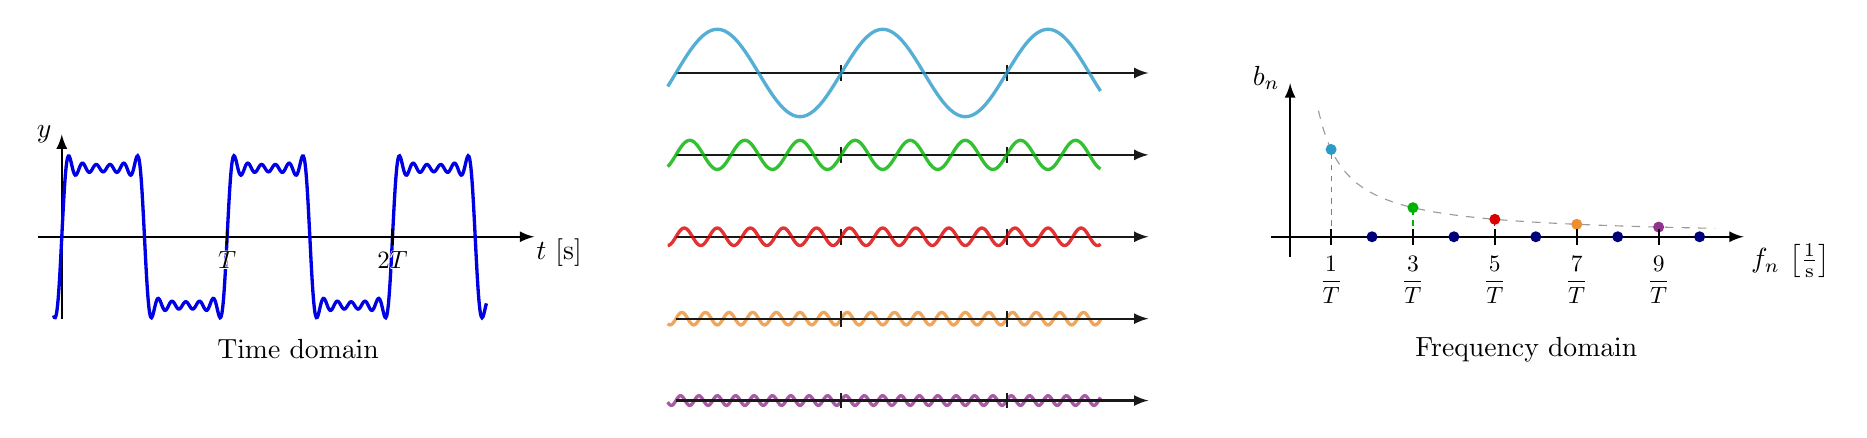
\begin{tikzpicture}

    % First plot
    \begin{scope}
        % Drawing lines
        \draw[->, thick] (-0.05*\xmax, 0) -- (\xmax,0) node[below right=-3] {$t$ [s]};
        \draw[->, thick] (0, \ymin) -- (0,\ymax) node[left] {$y$};
        \draw[xline, blue!90!black, very thick, samples=5*\N, smooth, variable=\t, domain=-0.05*\T:0.9*\xmax]
            plot(\t,{\f{1}+\f{3}+\f{5}+\f{7}+\f{9}+\f{11}},0); % node[above] {$f$};
         % Showing text
        \tick{{\T}, 0}{90} node[below=-1, scale=0.9] {\contour{white}{$T$}};
        \tick{{2*\T},0}{90} node[below=-1,scale=0.9] {\contour{white}{$2T$}};
        \node[scale=1] at (0.5*\xmax, -1.10*\ymax) {Time domain};
    \end{scope}

    % Second plot
    \begin{scope}[shift={(1.3*\xmax, 0)}]  
        \foreach \i/\col [evaluate={\z=\w*(\i - 5);}] in {9/mypurple, 7/myorange, 5/myred, 3/mygreen, 1/mycyan}{
            % Draw vertical lines
            \draw[black!90, thick] ({\T}, \z + 0.1) --++ (0, -0.2);  
            \draw[black!90, thick] ({2*\T},\z + 0.1) --++ (0, -0.2);
            % Draw horizontal arrows
            \draw[->, black!90, thick] (0, \z) --++ (\xmax, 0);  
            % Plot signals
            \draw[xline, \col, opacity=0.8, very thick, samples=5*\N, smooth, variable=\t, domain=-0.05*\T:0.9*\xmax]
                plot (\t, {-\z + 0.5*\f{\i}});
                }
    \end{scope}

    % Third plot
    \begin{scope}[shift={(2*1.3*\xmax, 0)}]  
        % Axis
        \draw[->,thick] (0, -0.2*\ymax) -- (0, 1.5*\ymax) node[above=2, left=0] {$b_n$};
        \draw[->,thick] (-0.04*\xmax, 0) --++ (\xmax, 0) node[below right=-1] {$f_n$ $\left[\frac{1}{\mathrm{s}}\right]$};
        % Text
        \node[scale=1] at (0.5*\xmax, -1.10*\ymax) {Frequency domain};
        % Dashed curve
        \draw[black!40, dashed, samples=3*\N, smooth, variable=\t, domain=0.06*\xmax:0.9*\xmax] plot(\t, {\A*4/pi/\t*\w}); 
        % Circles
        \foreach \i/\col [evaluate={\z=\w*\i;}] in {9/mypurple, 7/myorange, 5/myred, 3/mygreen, 1/mycyan}{
            \draw[\col,dash pattern=on 2 off 2] (\z, 0) --++ (0, {\A*4/pi/\i});
            \fill[\col] (\z, {\A*4/pi/\i}) circle(0.07);
           \tick{\z, 0}{90} node[below=1, scale=0.85] {$\dfrac{\i}{T}$};
           }
        \foreach \i [evaluate={\z=\w*\i;}] in {2, 4, ..., 10}{
          \fill[myblue!60!black] (\z, 0) circle(0.07);
          }
    \end{scope}
    
\end{tikzpicture}


\end{document}